\begin{IEEEbiography}
[{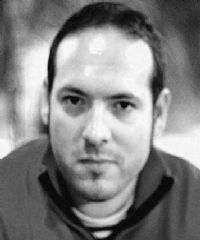
\includegraphics[width=1in,height=1.25in,clip,keepaspectratio]{images/placeholder_author.jpg}}]{Luis Felipe Borja-Borja} received a degree Computer Engineering in 2000 from the Central University (Ecuador) and received his PhD in Computer Science from the University of Alicante (Spain) in 2020. Since 2011, he has been a faculty member at the Faculty of Engineering and Applied Sciences at Universidad Central, where he is currently Professor and Director of the Computer Science degree. In addition, he has worked at the Graduate Institute of the same faculty as a tutor of some theses. His current research interests include computer vision, computational intelligence, machine learning, deep learning, and the analysis of human activity. In these lines of research, Dr. Borja has worked on a number of papers. 
\end{IEEEbiography}

\begin{IEEEbiography}
[{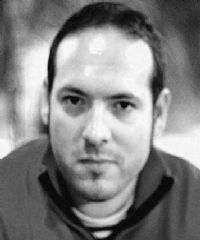
\includegraphics[width=1in,height=1.25in,clip,keepaspectratio]{images/placeholder_author.jpg}}]{Jorge Azorín-López} received a degree in Computer Engineering in 2001 and a Ph.D. degree in Computer Science at the University of Alicante (Spain) in 2007. Since 2001, he has been a faculty member of the Department of Computer Technology at the same university, where he is currently an Associate Professor and the Academic Secretary. His current research interests include 3D computer vision, computational intelligence, machine learning, deep learning, ambient intelligence, human activity analysis, and visual inspection. In these lines of research, Dr. Azorín has worked in 20 research projects (5 of them as coordinator) funded by national, regional, and local public and private entities. He has authored more than 100 contributions in several journals, conferences and book chapters. 
\end{IEEEbiography}

\begin{IEEEbiography}
[{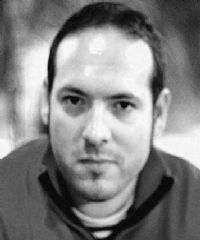
\includegraphics[width=1in,height=1.25in,clip,keepaspectratio]{images/placeholder_author.jpg}}]{Marcelo Saval-Calvo} is currently an Associate Professor at the University of Alicante. He obtained a degree in Computer Engineering from the University of Alicante in 2010, and a Master in 2011. He received his PhD in Computer Technology from the same university in 2015 funded with a public grant from the regional government of Valencian Community. His research focuses on 3D registration and reconstruction of deformable elements; sensorization for autonomous vehicles; and human behaviour analysis using artificial intelligence techniques. He has a collaboration with the University of Edinburgh that started in 2014 as part of his thesis research, later as a postdoctoral researcher for a year, and has continued until the present. He has participated in 6 research projects funded in competitive calls, being principal investigator of two of them. He has several publications in journals, most of them indexed in the JCR; 3 book chapters and 18 prestigious international conferences. He has supervised several undergrad and master thesis in both the University of Alicante and Edinburgh, and has been the phd co-supervisor of a student under an agreement between the University of Alicante and Central de Ecuador. Marcelo has been a reviewer for several international journals and conferences, and has been a member of the board of examiners for PhD, undergrad and master projects.
\end{IEEEbiography}

\begin{IEEEbiography}
[{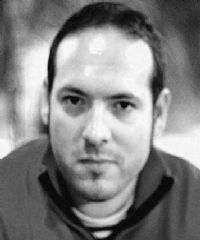
\includegraphics[width=1in,height=1.25in,clip,keepaspectratio]{images/placeholder_author.jpg}}]{Andrés Fuster-Guilló} received the B.S. degree in computer science engineering from the Polytechnic University of Valencia, Spain, in 1995, and the Ph.D. degree in computer science from the University of Alicante, Spain, in 2003. Since 1997, he has been a member of the faculty of the Department of Computer Science and Technology, University of Alicante, where he is currently an Associate Professor. He was a Deputy Coordinator of the Polytechnic School and the Director of the Secretariat for Information Technology, University of Alicante. During this period, he has coordinated and participated in several strategic technological projects, including Open University (transparency portal and open data), UACloud, and Smart University, among others. He has published over 80 articles in different areas of research, including computer vision, 3D vision, machine learning, artificial neural networks, and open data.
\end{IEEEbiography}


\begin{IEEEbiography}
[{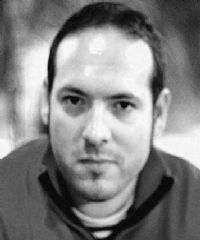
\includegraphics[width=1in,height=1.25in,clip,keepaspectratio]{images/placeholder_author.jpg}}]{Marc Sebban} received a Ph.D. in Machine Learning in 1996 from the Université of Lyon 1. After four years spent at the French West Indies and Guyana University as Assistant Professor, he got a position of Professor in 2002 at the University of Saint-Etienne (France). Since 2010, he was the head of the Machine Learning group and the director of the Computer Science, Cryptography and Imaging department of the Hubert Curien laboratory. Nowadays, he is the Deputy-director of the UMR CNRS Hubert Curien laboratory. His research interests focus on statistical learning theory, metric learning, representation Learning, transfer learning, optimal transport, theory of boosting and learning from highly imbalanced data.
\end{IEEEbiography}
